\documentclass[a4paper,10pt]{article}

\usepackage[utf8]{inputenc} % pour les accents
\usepackage[T1]{fontenc} % caracteres francais
\usepackage{geometry} %les marges
\usepackage[french]{babel} %langue principale
\usepackage[dvips]{graphicx}
\geometry{ hmargin=2cm, vmargin=2cm }

\pagestyle{empty} %pas de numerotation de page

%
% Debut du document
%
\begin{document}

\section*{FICHE DE VALIDATION DU LOGICIEL MASCARET V7P0}

\subsection*{Validation du noyau transcritique}

\subsection*{\emph{Validation de la propagation sur fond sec}}

\subsection*{Numéro du cas test : 20}

\subsection*{Auteur : Fabrice ZAOUI}


\vspace{1cm}

\subsection*{Description}

Considérons un barrage qui sépare un plan d'eau au repos d'une zone sèche. Au temps $t = 0\ s$, le barrage est retiré. Le problème est de déterminer l'écoulement qui en résulte.

Dans le cas o\`{u} le canal est rectangulaire à fond plat et sans frottement, il est possible de déterminer la solution analytique du problème\footnote{A. Ritter,\emph{Die Fortplanzung der Wasserwellen}, Z Verdeut. Ing 36, 1892}. Ce cas est intéressant car il permet de valider le schéma numérique sur un cas de propagation d'onde sur fond sec, ce qui est une première étape indispensable si l'on veut traiter des calculs d'onde de submersion (propagation de l'onde de submersion dans une vallée sèche).

\subsection*{Données géométriques}

Le calcul est réalisé dans un canal de $5000\ m$ de longueur, dont chaque profil en travers est un rectangle de largeur constante et égale à $1\ m$. La cote du fond est constante.

\subsection*{Données physiques}

\begin{itemize} 
 \item Conditions aux limites : débit nul à l'amont, cote nulle à l'aval;
 \item Frottement : nul;
 \item Conditions initiales :
 \begin{itemize}
  \item cote $= 6\ m$ pour $x < 2000\ m$;
  \item cote $= 10^{-6}\ m$ pour $x >= 2000\ m$.
 \end{itemize}
\end{itemize} 

Remarque : la hauteur d'eau à l'aval n'est pas mise à zéro mais à une valeur faible pour éviter des problèmes numériques.

\subsection*{Données numériques}

\begin{itemize}
 \item Pas d'espace régulier égal à $5\ m$;
 \item Pas de planimétrage égal à $0.5\ m$;
 \item Pas de temps de $0.08\ s$;
 \item Durée de simulation de $200\ s$.
\end{itemize}


\subsection*{Résultats}

Sur les figures~\ref{fig1} et \ref{fig2} sont comparés la hauteur d'eau et le débit calculés avec la hauteur d'eau et le débit analytiques. On note une bonne concordance entre les variables calculées et analytiques. La zone de front est bien représentée. On remarque la formation d'un choc très faible au lieu d'avoir une hauteur d'eau parfaitement tangente à la cote du fond. On note également une diffusion lorsque l'onde de détente se raccorde avec l'état de gauche (cote égale à $6\ m$).




\newpage

\begin{figure}
 \begin{center}
  \includegraphics[angle=270,width=15cm]{Hauteur.eps}
  \caption{Hauteurs d'eau comparées en fin de simulation}
  \label{fig1}
 \end{center}
\end{figure}

\begin{figure}
 \begin{center}
  \includegraphics[angle=270,width=15cm]{Debit.eps}
  \caption{Débits comparés en fin de simulation}
  \label{fig2}
 \end{center}
\end{figure}




%
% fin du document
%
\end{document}          
